
\newcommand{\E}{\mathbf{E}}
\newcommand{\B}{\mathbf{B}}
\renewcommand{\H}{\mathbf{H}}
\newcommand{\D}{\mathbf{D}}

\newcommand{\J}{\mathbf{J}}
\newcommand{\Jphat}{\hat{\J}_p}
\newcommand{\Jpol}{\J^p}
\newcommand{\JpolScalar}{J^p}
\newcommand{\plasfreq}{\omega_p}
\newcommand{\plasfreqtilde}{\tilde{\omega}_p}

\newcommand{\xbf}{\mathbf{x}}

\newcommand{\xbftilde}{\tilde{\mathbf{x}}}
\newcommand{\nablatilde}{\tilde{\nabla}}
\newcommand{\Etilde}{\tilde{\mathbf{E}}}
\newcommand{\Btilde}{\tilde{\mathbf{B}}}
\newcommand{\Htilde}{\tilde{\mathbf{H}}}
\newcommand{\Dtilde}{\tilde{\mathbf{D}}}
\newcommand{\Jtilde}{\tilde{\mathbf{J}}}
\newcommand{\Jtildep}{\tilde{\mathbf{J}}_P}
\newcommand{\ttilde}{\tilde{t}}
\renewcommand{\t}{t}
\newcommand{\omegatilde}{\tilde{\omega}}
\newcommand{\gammatilde}{\tilde{\gamma}}

\newcommand{\bigO}{\mathcal{O}}
\newcommand{\Epsilon}{\mathcal{E}}

\newcommand{\weightfunc}{\mathbf{W}}
\newcommand{\R}{\mathbf{R}}
\newcommand{\ut}{\frac{\partial \mathbf{U}}{\partial t}}
\newcommand{\fk}{\frac{\partial \mathbf{F_k (\mathbf{U})} }{\partial x_k}}

% --------------------------------------------------------------------------------------------- %
% General
% --------------------------------------------------------------------------------------------- %

\newcommand{\Real}{\mathbb{R}}
\newcommand{\norm}[1]{\left\lVert#1\right\rVert}
\newcommand{\zerov}{\mathbf{0}_3}
\newcommand{\IdentityVect}{\mathbf{I}_3}
\newcommand{\nsd}{\textrm{nsd}}

% --------------------------------------------------------------------------------------------- %
% Physical Problem
% --------------------------------------------------------------------------------------------- %

% conservation form maxwells
\newcommand{\USoltn}{\mathbf{U}}
\newcommand{\Flux}{\mathbf{F}}
\newcommand{\maxwellSource}{\mathbf{S}}
\newcommand{\eps}{\varepsilon}

% Quasilinear form
\newcommand{\AQuasiLinear}{\mathbf{A}}
\newcommand{\RQuasiL}{\mathbf{R}}
\newcommand{\RTot}{\mathbf{R}^{s}}
\newcommand{\AQuasiLinearComb}{\AQuasiLinear^{s}}

% Quasilinear form TE/TM
\newcommand{\Jnormalised}[1]{J_{#1}^*} % scalar

% Compact Form
\newcommand{\waveNumberVectZ}{\mathbf{k}_z}
\newcommand{\waveNumberZ}{k_z}
\newcommand{\phase}{\phi}

% integral formulation of Maxwell's equations
\newcommand{\vectdl}{\mathrm{d}\boldsymbol{\ell}}
\newcommand{\vectdS}{\mathrm{d}\mathbf{S}}
\newcommand{\Vol}{V}
\newcommand{\dV}{\mathrm{d}V}

% Physical Problem - dimensionless units
\newcommand{\czero}{c_0}
\newcommand{\charLen}{l}
\newcommand{\intImpFS}{\sqrt{\frac{\mu_0}{\eps_0}}} % ininsic impedence free space (\eta_0)

% Constitutive equations
\newcommand{\ElecSuccept}{\chi}
\newcommand{\MagSuccept}{\chi^{m}}
\newcommand{\Ptilde}{\tilde{\mathbf{P}}}
\newcommand{\Mtilde}{\tilde{\mathbf{M}}}

% Drude model - ADE
\newcommand{\PtildeInf}{\tilde{\mathbf{P}}_{\infty}}
\newcommand{\PtildeElec}{\tilde{\mathbf{P}}_P}
\newcommand{\PtildeInfFreq}{\hat{\tilde{\mathbf{P}}}_{\infty}}
\newcommand{\PtildeElecFreq}{\hat{\tilde{\mathbf{P}}}_P}
\newcommand{\ElecSucceptInf}{\chi_{\infty}}
\newcommand{\DInf}{\D_{\infty}}
\newcommand{\DtildeInf}{\tilde{\D}_{\infty}}

% Drude Model - mechanical
\newcommand{\xdispelecvect}{\tilde{\mathbf{x}}_e}
\newcommand{\EappliedDrude}{\tilde{\mathbf{E}}_{app}}

% Helmholtz
\newcommand{\EHelm}{\E_0}
\newcommand{\HHelm}{\H_0}


% --------------------------------------------------------------------------------------------- %
% PDEs and ODEs
% --------------------------------------------------------------------------------------------- %

\newcommand{\dpart}[2][]{\frac{\partial}{\partial#2} #1}
\newcommand{\dpartt}[1]{\frac{\partial}{\partial t} #1}
\newcommand{\ddpartt}[1][]{\frac{\partial^2}{\partial t^2} #1}
\newcommand{\dpartttilde}[1]{\frac{\partial}{\partial \tilde{t} } #1}
\newcommand{\dpartx}[1]{\frac{\partial}{\partial x} #1}
\newcommand{\dpartxtilde}[1]{\frac{\partial}{\partial \tilde{x}} #1}

\newcommand{\dode}[2][]{\frac{d}{d#2} #1}
\newcommand{\dodet}[1]{\frac{d}{d t} #1}
\newcommand{\dodett}[1][]{\frac{d^2}{d t^2} #1}
\newcommand{\dodettilde}[1]{\frac{d}{d \tilde{t}} #1}
\newcommand{\dodex}[1]{\frac{d}{d x} #1}
\newcommand{\dodextilde}[1]{\frac{d}{d \tilde{x}} #1}
% --------------------------------------------------------------------------------------------- %
% Figures
% --------------------------------------------------------------------------------------------- %

\newcommand{\singleFigure}[3]{
\begin{figure}[htbp!]
  \begin{center}
    \includegraphics[width=\textwidth]{Figures/#1}
  \end{center}
  \caption{#2}
  \label{fig:#3}
\end{figure}
}

\newcommand{\FigTwoByOne}[6]{
\centering
\begin{subfigure}{0.495\textwidth}
  \centering
  \includegraphics[width=\textwidth]{Figures/#1}
  \caption{#3}
  \label{fig:#5}
\end{subfigure} %
\begin{subfigure}{0.495\textwidth}
  \centering
  \includegraphics[width=\textwidth]{Figures/#2}
  \caption{#4}
  \label{fig:#6}
\end{subfigure}
}

\newcommand{\seperateFiguresSetSideBySide}[3]{
\begin{figure}
\centering
\begin{minipage}{.45\linewidth}
  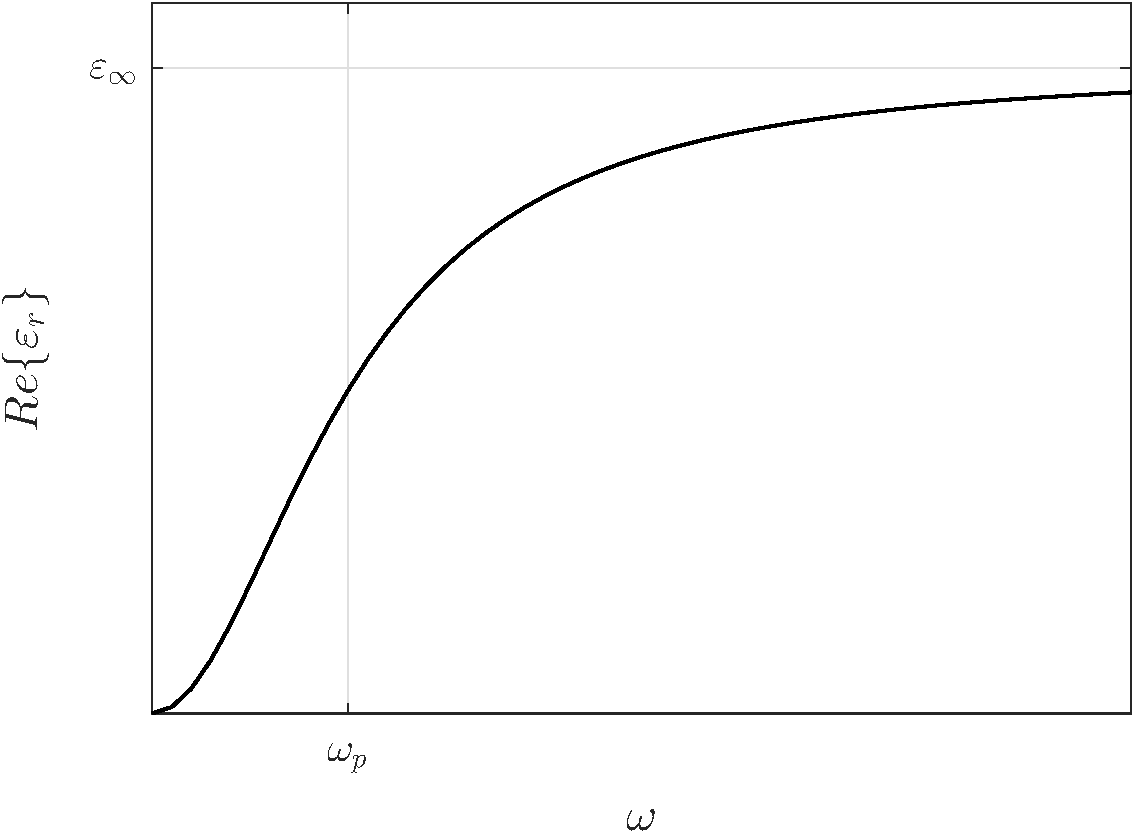
\includegraphics[width=\linewidth]{Figures/Chapters/PhysicalProblem/drudePermittivityReal}
  \captionof{figure}{First caption}
  \label{img1}
\end{minipage}
\hspace{.05\linewidth}
\begin{minipage}{.45\linewidth}
  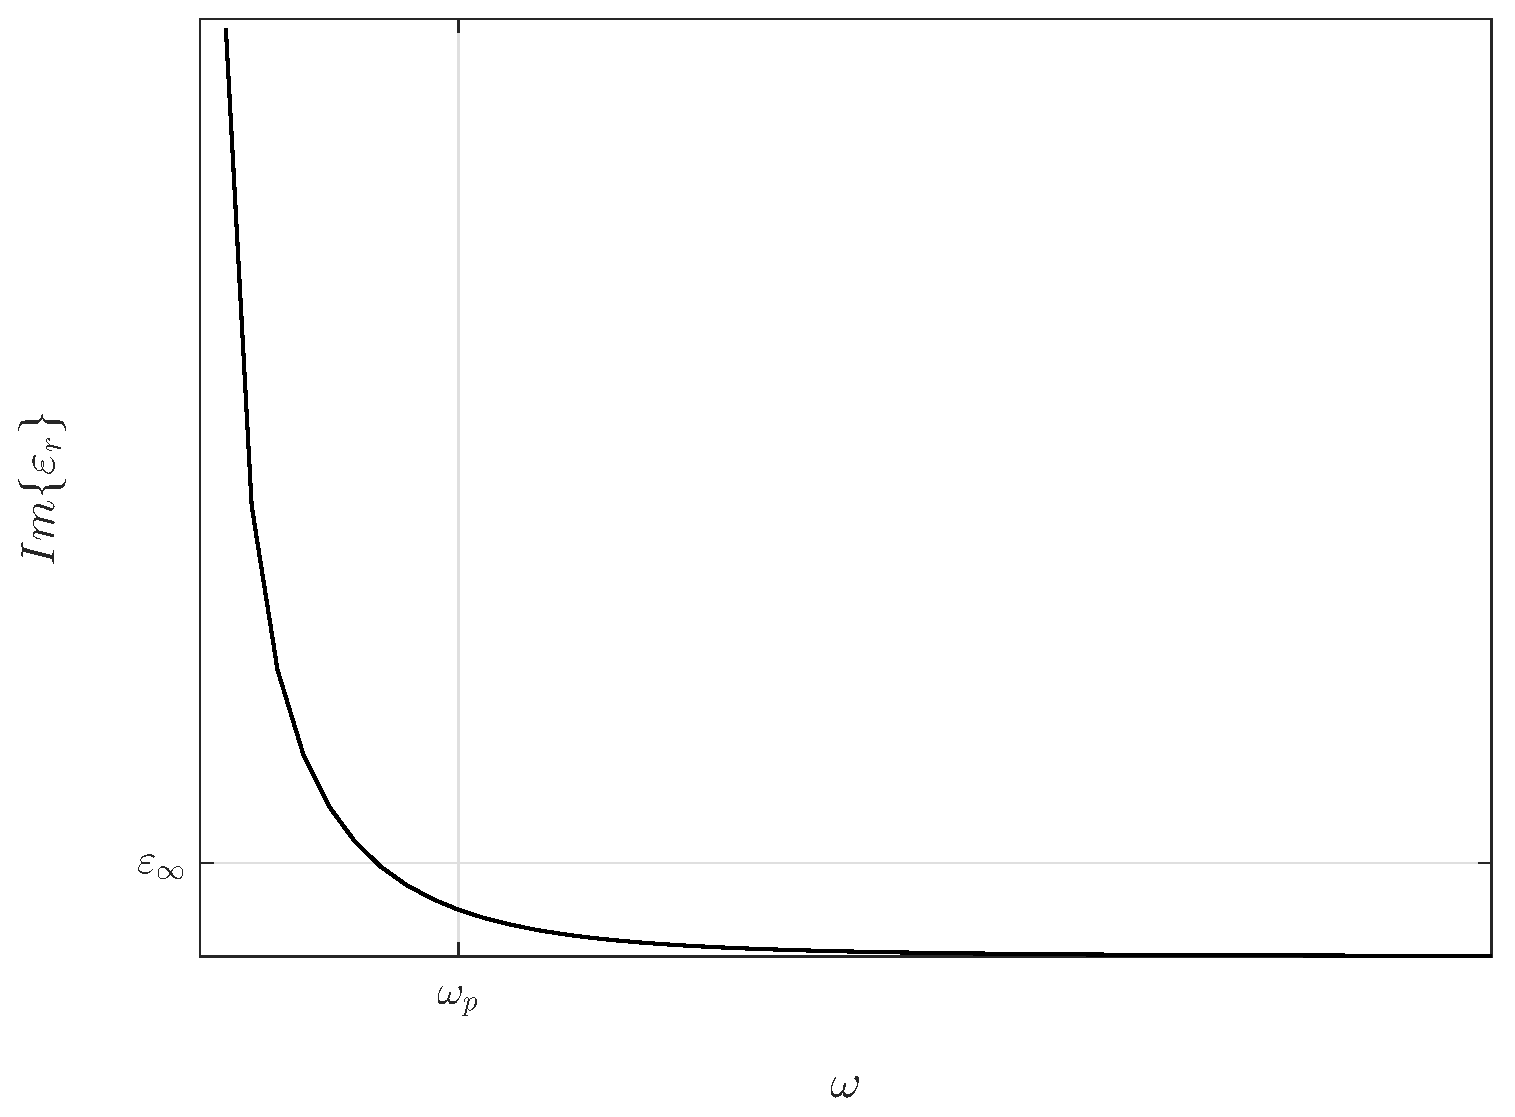
\includegraphics[width=\linewidth]{Figures/Chapters/PhysicalProblem/drudePermittivityImag}
  \captionof{figure}{Second caption}
  \label{img2}
\end{minipage}
\end{figure}
}


\usepackage{xparse}

\ExplSyntaxOn
% Usage:
% \twoimages{
%     {Chapters/figure/path}{figure caption},
%     {Chapters/figure/path}{another caption}
% }
\NewDocumentCommand{\twoimages}{ >{ \SplitList {,} } m }
 {
  \centering
  \ProcessList { #1 } { \__davs_process_argument:n }
 }
\cs_new_protected:Nn \__davs_process_argument:n
 {
  \__davs_image:nnn #1
 }
\cs_new_protected:Nn \__davs_image:nnn
 {
  \begin{subfigure}{0.45\textwidth}
    \centering
    \includegraphics[width=\textwidth]{Figures/#1}
    %\caption{#2}
    %\label{ris:#1}
  \end{subfigure} %
  \hfill
  \penalty0 % we provide a break point
 }
\ExplSyntaxOff
%%% Local Variables:
%%% mode: latex
%%% TeX-master: t
%%% End:
